\section{Method}
\label{sec:method}

% \begin{figure*}[t]
  \centering
  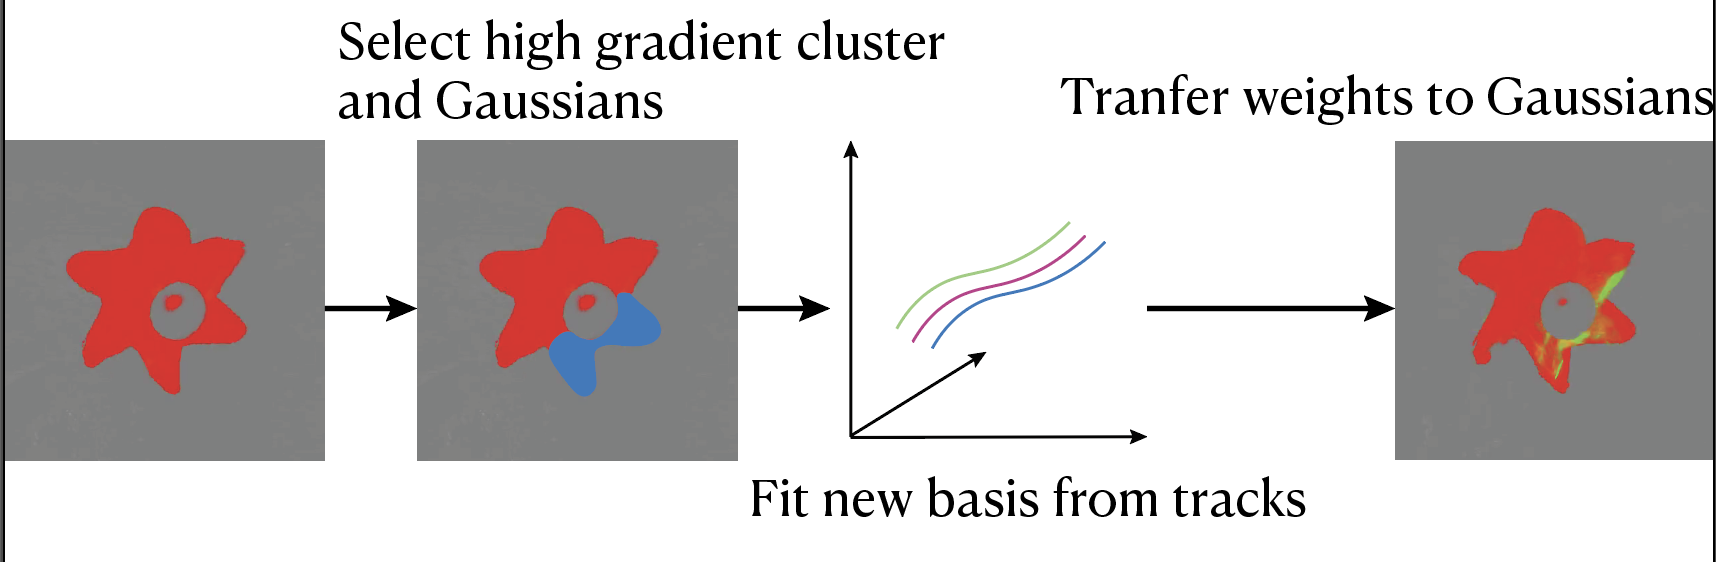
\includegraphics[width=\linewidth]{img/pipeline-draft.png}
  \caption{Overview of our adaptive motion basis densification pipeline.}
  \label{fig:pipeline}
\end{figure*}

\begin{figure*}[t]
  \centering
  \setlength{\tabcolsep}{1pt}
  \begin{tabular}{@{}c@{\hspace{2pt}}ccccc@{}}
    \rotatebox{90}{\makebox[0.247\linewidth][c]{\footnotesize Apple}} &
      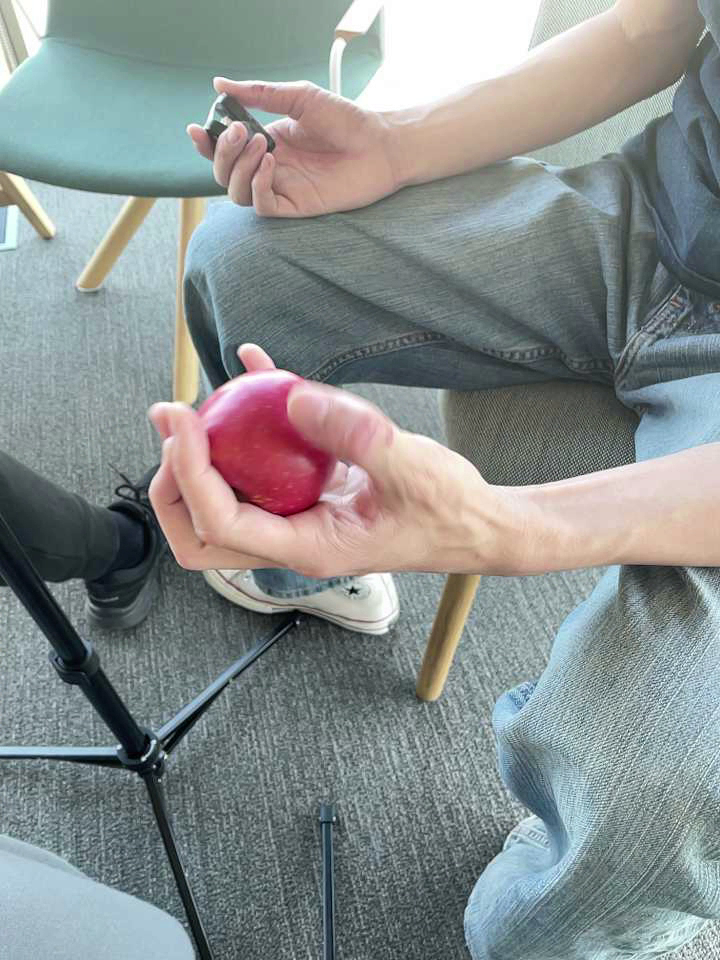
\includegraphics[width=0.185\linewidth]{img/comparison/apple_gt.png} &
      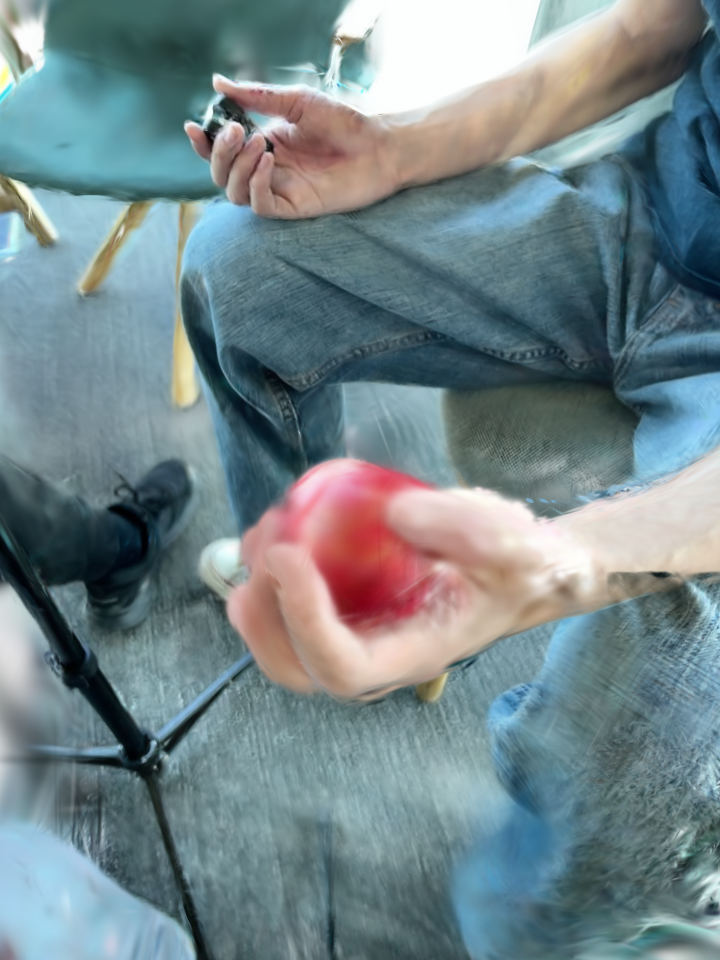
\includegraphics[width=0.185\linewidth]{img/comparison/apple_ours.png} &
      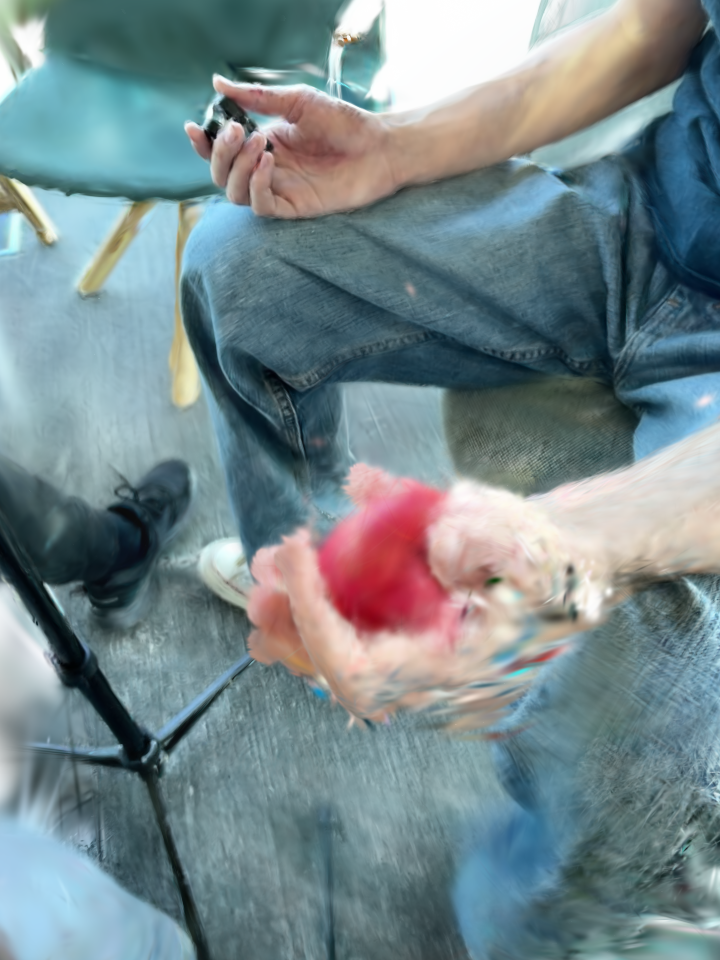
\includegraphics[width=0.185\linewidth]{img/comparison/apple_som.png} &
      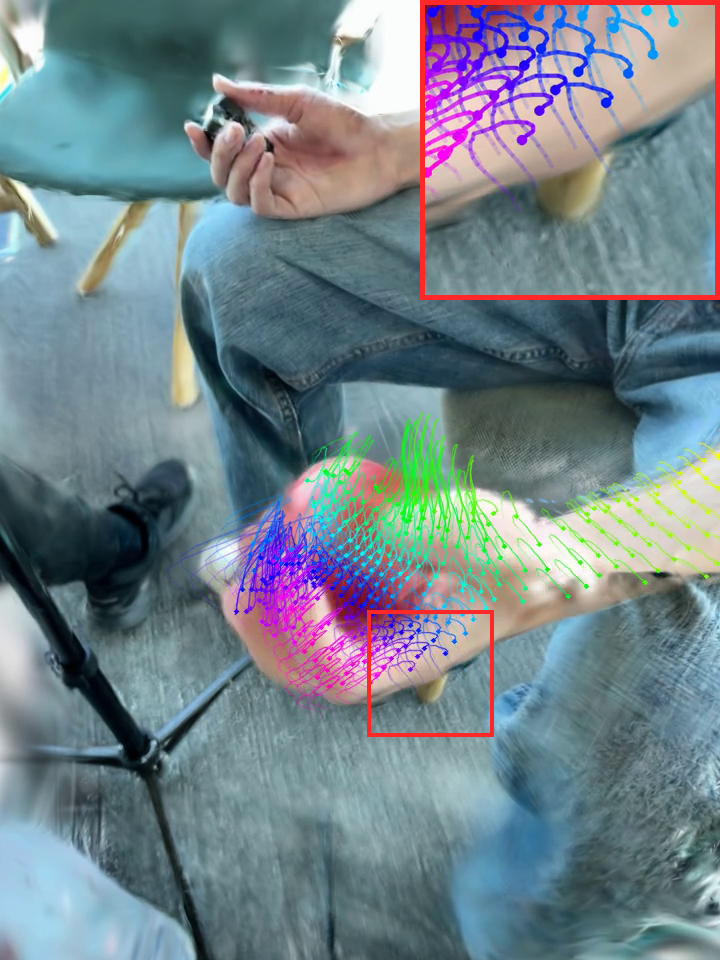
\includegraphics[width=0.185\linewidth]{img/comparison/apple_ours_tracks.png} &
      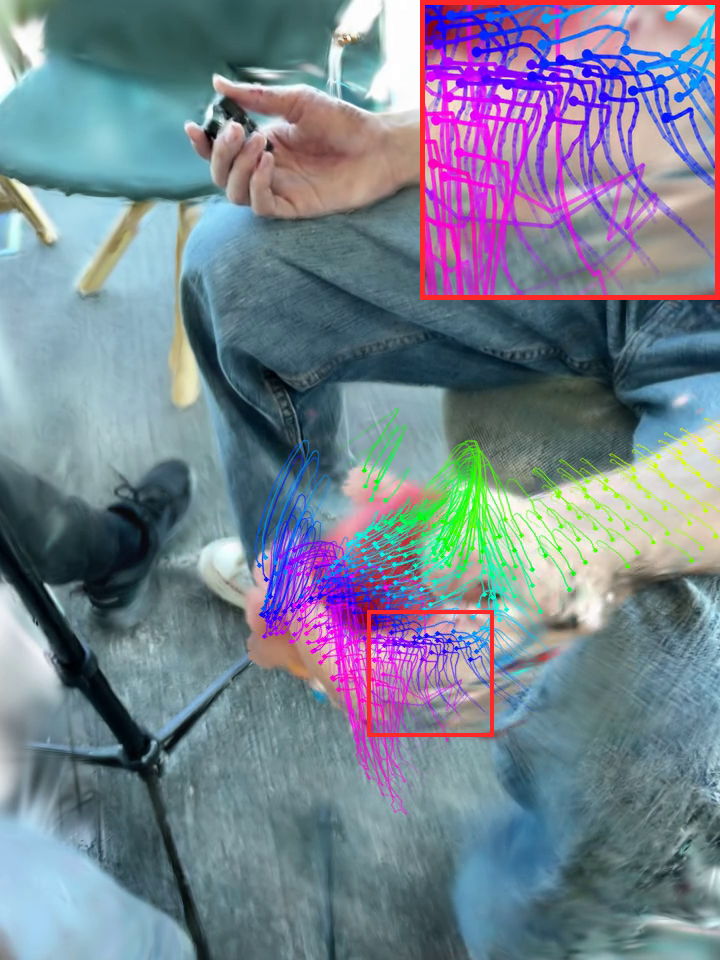
\includegraphics[width=0.185\linewidth]{img/comparison/apple_som_tracks.png} \\
    \rotatebox{90}{\makebox[0.247\linewidth][c]{\footnotesize Paper Windmill}} &
      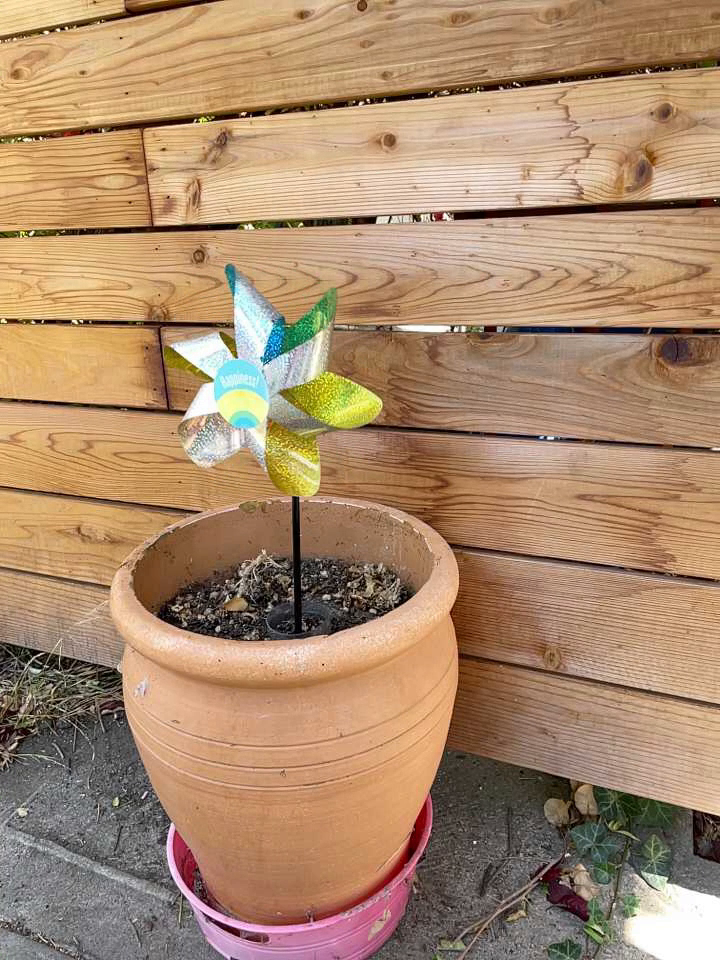
\includegraphics[width=0.185\linewidth]{img/comparison/windmill_gt.png} &
      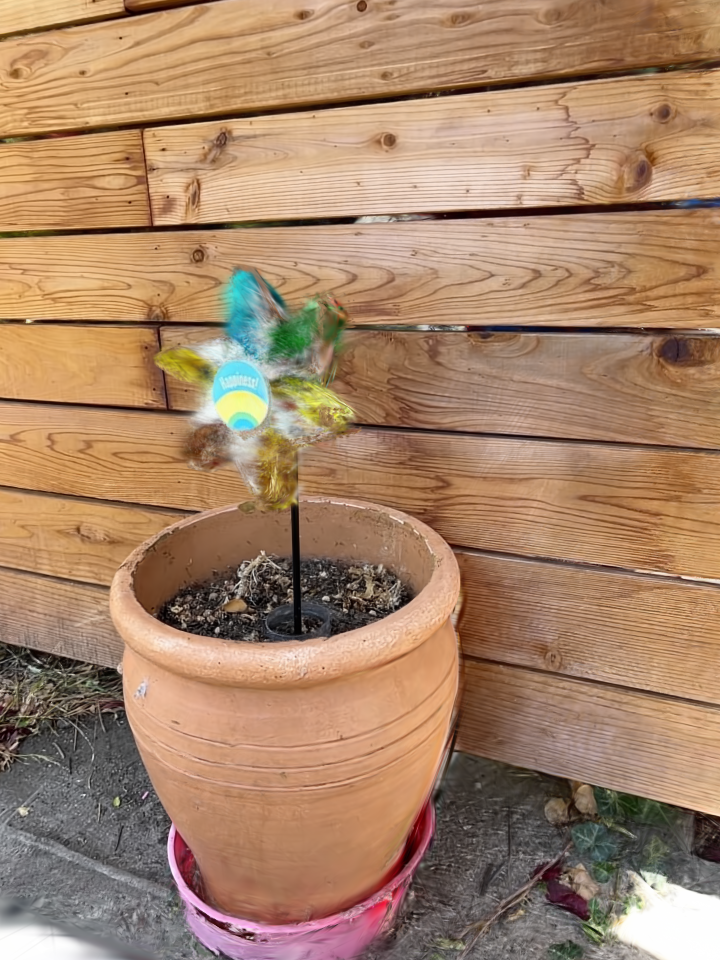
\includegraphics[width=0.185\linewidth]{img/comparison/windmill_ours.png} &
      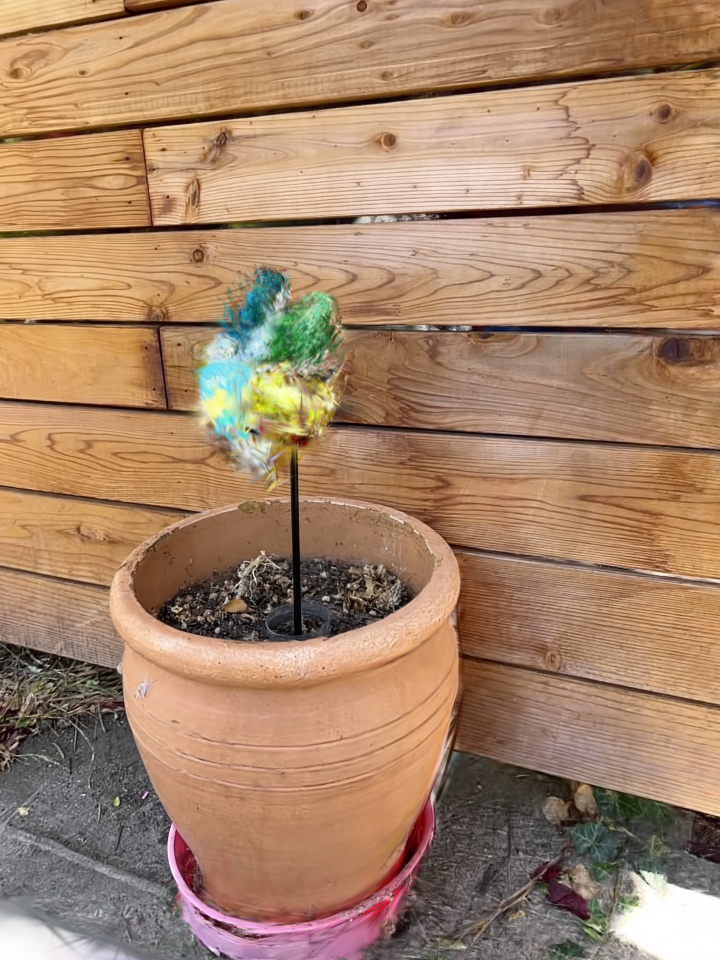
\includegraphics[width=0.185\linewidth]{img/comparison/windmill_som.png} &
      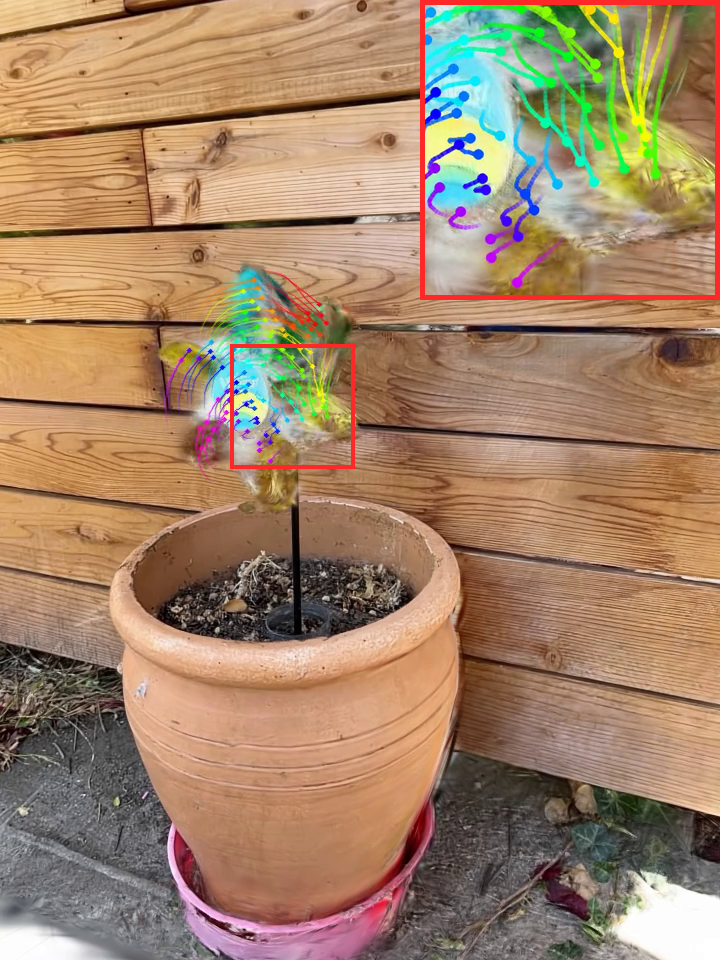
\includegraphics[width=0.185\linewidth]{img/comparison/windmill_ours_tracks.png} &
      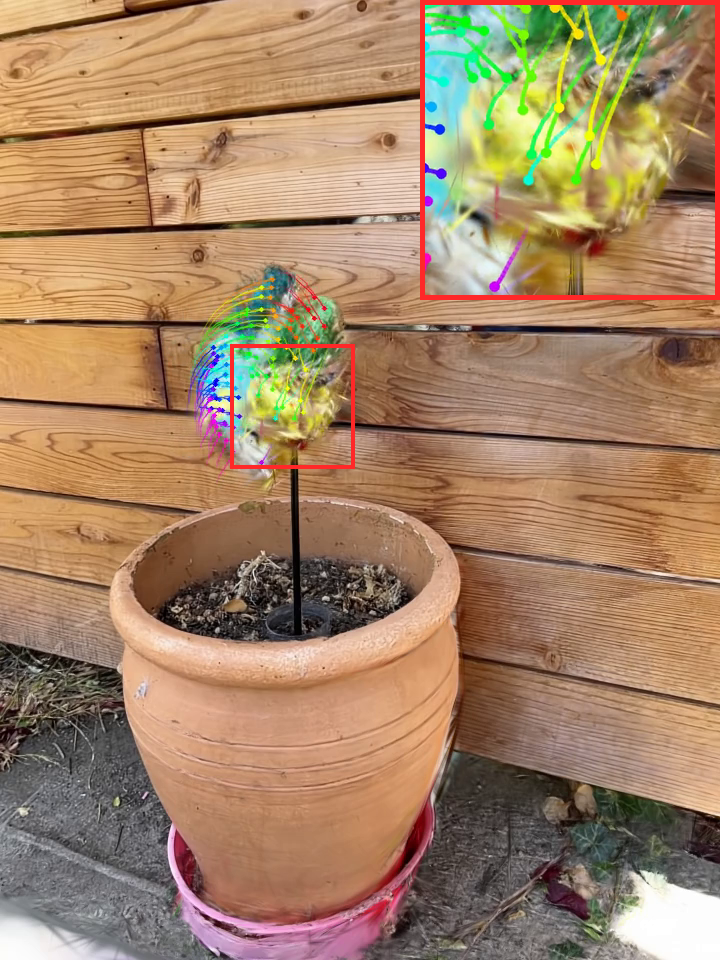
\includegraphics[width=0.185\linewidth]{img/comparison/windmill_som_tracks.png} \\
    
     & \makebox[0.185\linewidth][c]{\footnotesize GT (Test View)} &
       \makebox[0.185\linewidth][c]{\footnotesize Ours} &
       \makebox[0.185\linewidth][c]{\footnotesize SoM} &
       \makebox[0.185\linewidth][c]{\footnotesize Ours (Tracks)} &
       \makebox[0.185\linewidth][c]{\footnotesize SoM (Tracks)} \\
  \end{tabular}
 \caption{\lulu{Replace with updated visualizations + all the baselines}Our method retains regularization toward the main motion modes, while SoM overfits and degrades on the test view.}
  \label{fig:qualitative-comparison}
\end{figure*}
  % results figure (two columns): input here so it lands before the references
% [Claude] 2026-11-05: the per-scene tables moved to the supplementary, sec/X_suppl.tex (user request).
% % Claude, generated by tests/candidate_full_tables.py --fmt tex --ds iPhone --ours split_init --partial (branch momo-modes; ours = MoMo = L2 + clustering + 5 % cutoff, no children; block B 10, user 2026-11-04); orange = not yet accepted.
\begin{table*}[t]
  \centering
  \footnotesize
  \setlength{\tabcolsep}{4pt}
  \begin{tabular}{@{}lcccccccccc@{}}
    \toprule
     & & \multicolumn{3}{c}{PSNR\,$\uparrow$} & \multicolumn{3}{c}{SSIM\,$\uparrow$} & \multicolumn{3}{c}{LPIPS\,$\downarrow$} \\
    \cmidrule(lr){3-5} \cmidrule(lr){6-8} \cmidrule(l){9-11}
    Scene & $B$ & SoM-10 & SoM-$B$ & Ours & SoM-10 & SoM-$B$ & Ours & SoM-10 & SoM-$B$ & Ours \\
    \midrule
    apple & 5 & \textbf{16.38} & 16.28 & 16.36 & 0.744 & 0.744 & \textbf{0.747} & 0.525 & 0.525 & \textbf{0.518} \\
    teddy & 8 & 13.94 & 14.06 & \textbf{14.09} & 0.558 & 0.561 & \textbf{0.562} & 0.509 & 0.512 & \textbf{0.506} \\
    spin & 9 & \textbf{17.27} & 17.14 & 17.10 & \textbf{0.697} & 0.696 & 0.695 & 0.294 & 0.296 & \textbf{0.292} \\
    paper-windmill & 9 & 19.55 & \textbf{19.57} & 19.55 & \textbf{0.553} & \textbf{0.553} & 0.552 & 0.200 & \textbf{0.198} & 0.200 \\
    block & 10 & \textbf{16.93} & \textbf{16.93} & 16.83 & \textbf{0.638} & \textbf{0.638} & \textbf{0.638} & \textbf{0.417} & \textbf{0.417} & 0.418 \\
    \midrule
    Average & 8.2 & \textbf{16.81} & 16.79 & 16.79 & 0.638 & 0.638 & \textbf{0.639} & 0.389 & 0.390 & \textbf{0.387} \\
    \bottomrule
  \end{tabular}
  \caption{\claudetag\ Metrics on the covisible pixels (the dataset's covisibility masks, as in DyCheck) on the held-out views of DyCheck (iPhone)~\cite{gao2022dynamic}, per scene: ours
    (\cref{sec:split-init}) against SoM~\cite{wang2025shape} with its default 10 bases (SoM-10) and with as many bases
    as ours (SoM-$B$). $B$: number of bases of our method, chosen by its $\tau = 0.05$ cutoff. Mean over three seeds; last row: average over the scenes.
    Best value in bold. }
  \label{tab:full-dycheck}
\end{table*}
  % results tables (two columns), same reason
% % Claude, generated by tests/candidate_full_tables.py --fmt tex --ds NVIDIA --ours split_init --partial (branch momo-modes; ours = L2 + clustering, no children); orange = not yet accepted.
% Claude 2026-11-05: Umbrella at the 5 % rule's B = 6 (all three seeds; ours + SoM-6 trained on Killarney, outputs/bdf_killarney,
% linked into outputs/bdf), so every row is at the rule's B. Rows other than Umbrella and Average unchanged by the regeneration.
\begin{table*}[t]
  \centering
  \footnotesize
  \setlength{\tabcolsep}{4pt}
  \begin{tabular}{@{}lcccccccccc@{}}
    \toprule
     & & \multicolumn{3}{c}{PSNR\,$\uparrow$} & \multicolumn{3}{c}{SSIM\,$\uparrow$} & \multicolumn{3}{c}{LPIPS\,$\downarrow$} \\
    \cmidrule(lr){3-5} \cmidrule(lr){6-8} \cmidrule(l){9-11}
    Scene & $B$ & SoM-10 & SoM-$B$ & Ours & SoM-10 & SoM-$B$ & Ours & SoM-10 & SoM-$B$ & Ours \\
    \midrule
    Balloon1 & 4 & \textbf{23.89} & \textbf{23.89} & 23.86 & 0.793 & \textbf{0.794} & 0.792 & \textbf{0.058} & 0.059 & 0.060 \\
    Balloon2 & 6 & \textbf{23.97} & 23.91 & 23.93 & \textbf{0.831} & 0.830 & \textbf{0.831} & \textbf{0.073} & 0.074 & 0.074 \\
    Jumping & 8 & \textbf{20.22} & 20.19 & 20.11 & \textbf{0.701} & 0.700 & 0.696 & \textbf{0.143} & 0.145 & 0.150 \\
    Playground & 7 & \textbf{17.03} & 17.01 & 17.00 & \textbf{0.553} & \textbf{0.553} & \textbf{0.553} & \textbf{0.158} & 0.162 & 0.162 \\
    Skating & 5 & \textbf{27.87} & 27.81 & 27.75 & \textbf{0.914} & \textbf{0.914} & 0.912 & \textbf{0.048} & 0.049 & 0.050 \\
    Truck & 6 & 27.56 & 27.58 & \textbf{27.76} & 0.876 & 0.877 & \textbf{0.878} & 0.052 & 0.052 & \textbf{0.049} \\
    Umbrella & 6 & 23.23 & 23.22 & \textbf{23.25} & \textbf{0.572} & \textbf{0.572} & 0.571 & \textbf{0.168} & \textbf{0.168} & 0.170 \\
    \midrule
    Average & 6.0 & \textbf{23.40} & 23.37 & 23.38 & \textbf{0.749} & 0.748 & 0.748 & \textbf{0.100} & 0.101 & 0.102 \\
    \bottomrule
  \end{tabular}
  \caption{\claudetag\ Metrics on the covisible pixels (the dataset's covisibility masks, as in DyCheck) on the held-out views of NVIDIA Dynamic Scenes~\cite{yoon2020novel}, per scene: ours
    (\cref{sec:split-init}) against SoM~\cite{wang2025shape} with its default 10 bases . $B$: number of bases of our method, chosen by its $\tau = 0.05$ cutoff. Mean over three seeds; last row: average over the scenes.
    Best value in bold. }
  \label{tab:full-nvidia}
\end{table*}


% [Claude] 2026-11-05: preliminaries subsection drafted (user request).
\subsection{Preliminaries: 3D Gaussian Splatting}
\label{sec:prelim}
3D Gaussian Splatting (3DGS)~\cite{kerbl20233d} represents a scene as a set of anisotropic 3D Gaussians.
Each Gaussian $g$ has a center $\boldsymbol{\mu}_g$, a rotation $\mathbf{R}_g$ and per-axis scales $\mathbf{s}_g$, which give its covariance $\boldsymbol{\Sigma}_g = \mathbf{R}_g \operatorname{diag}(\mathbf{s}_g)^2 \mathbf{R}_g^\top$, as well as an opacity $o_g$ and a color $\mathbf{c}_g$.
A view is rendered by projecting the Gaussians onto the image plane, sorting them by depth and alpha-compositing them front to back,
\begin{equation}
  \mathbf{C}(\mathbf{p}) = \sum_{i} \mathbf{c}_i\, \alpha_i \prod_{j<i} (1 - \alpha_j) ,
  \label{eq:3dgs}
\end{equation}
where $\alpha_i$ is the opacity $o_i$ times the projected 2D Gaussian of $i$ evaluated at pixel $\mathbf{p}$.
Since the rasterization is differentiable, all parameters are optimized with a photometric loss on the input images.
For a dynamic scene, SoM~\cite{wang2025shape} defines the Gaussians in a canonical frame $t_0$ and moves their centers and rotations over time (\cref{sec:split-init}).

% [Claude] 2026-11-05: "Motion Bases Analysis" moved to sec/3_analysis.tex as 3.2 (user request); here its heading and figure inputs are commented out and its text is struck.
% \subsection{Motion Bases Analysis}
% % Was an inline wrapfigure in sec/4_method.tex (workshop version); caption = its commented-out caption.
\begin{figure}[t]
  \centering
  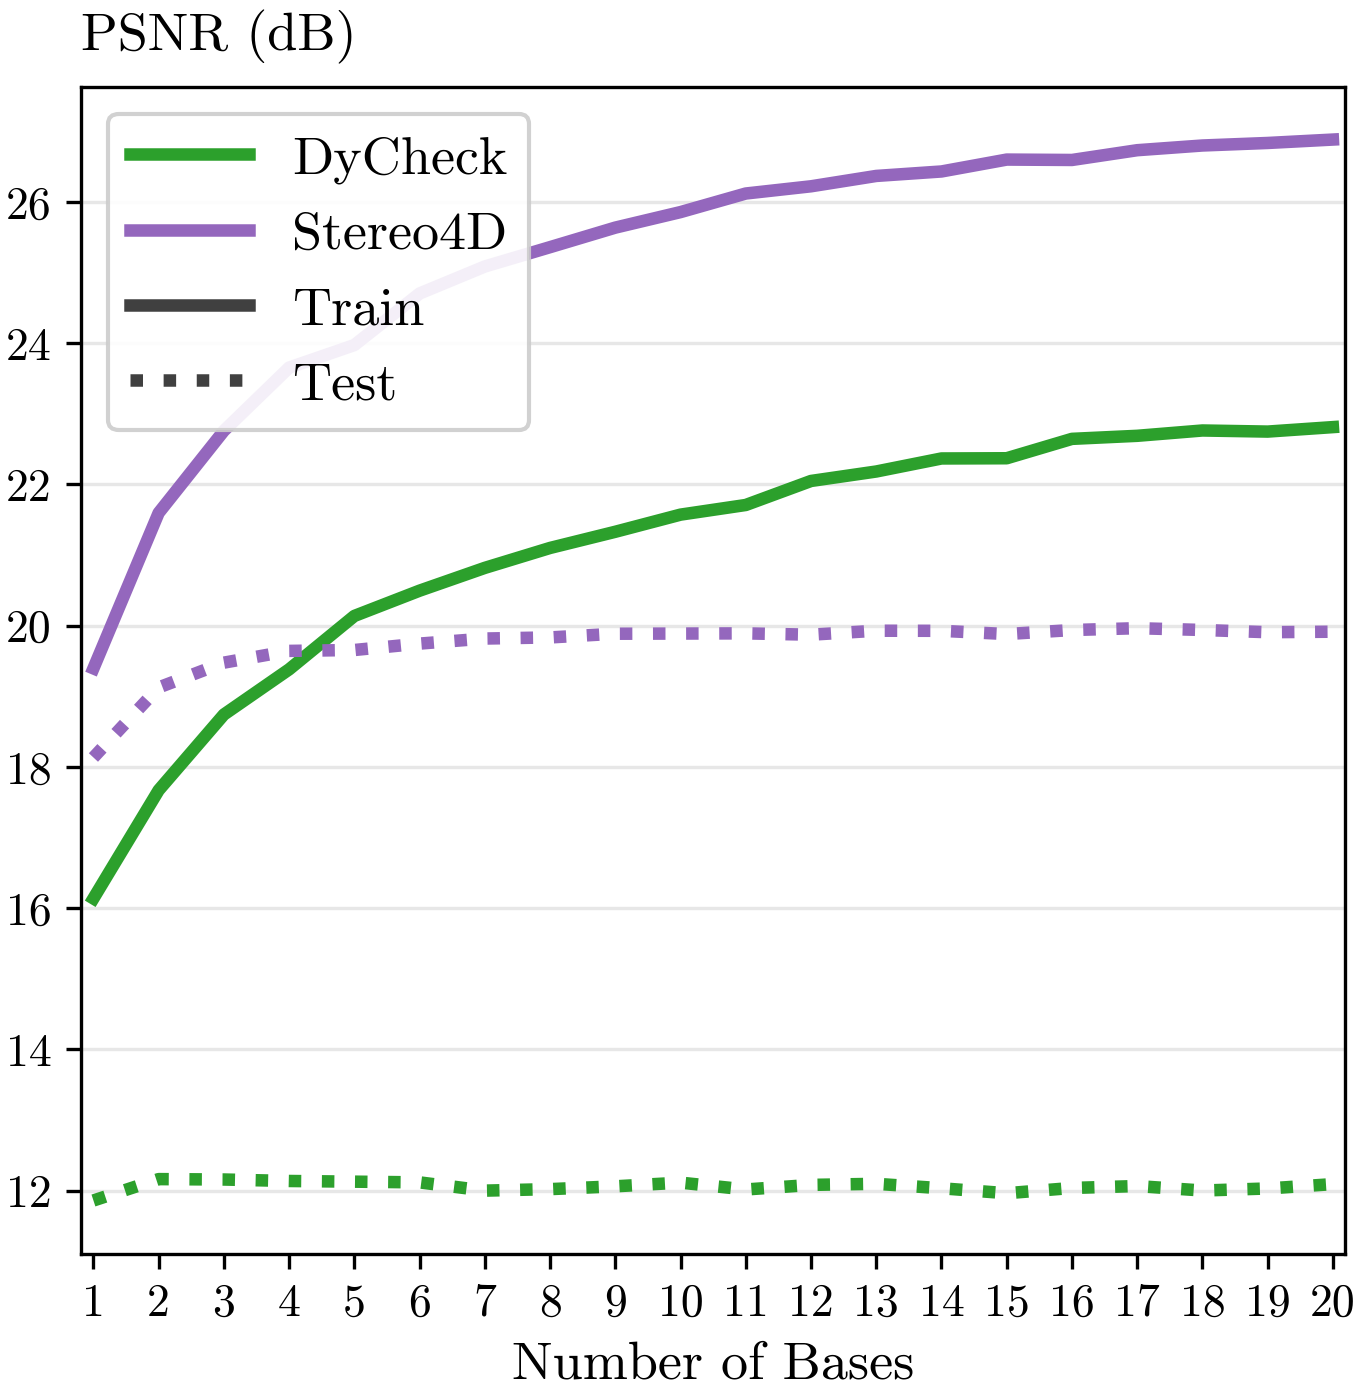
\includegraphics[width=0.75\linewidth]{img/combined-sweep.png}
  \caption{Training PSNR rises with more bases, while test PSNR quickly saturates. \lulu{Replace with NVIDIA instead of stereo}}
  \label{fig:basis-psnr}
\end{figure}

%The Stereo4D dataset presents an easier benchmark due to the high overlap between the training and validation views.

% % Was a commented-out wrapfigure in sec/4_method.tex (workshop version); caption = its commented-out caption.
% Label renamed from fig:basis-utilization, which fig/synthetic_weights.tex uses.
\begin{figure}[t]
  \centering
  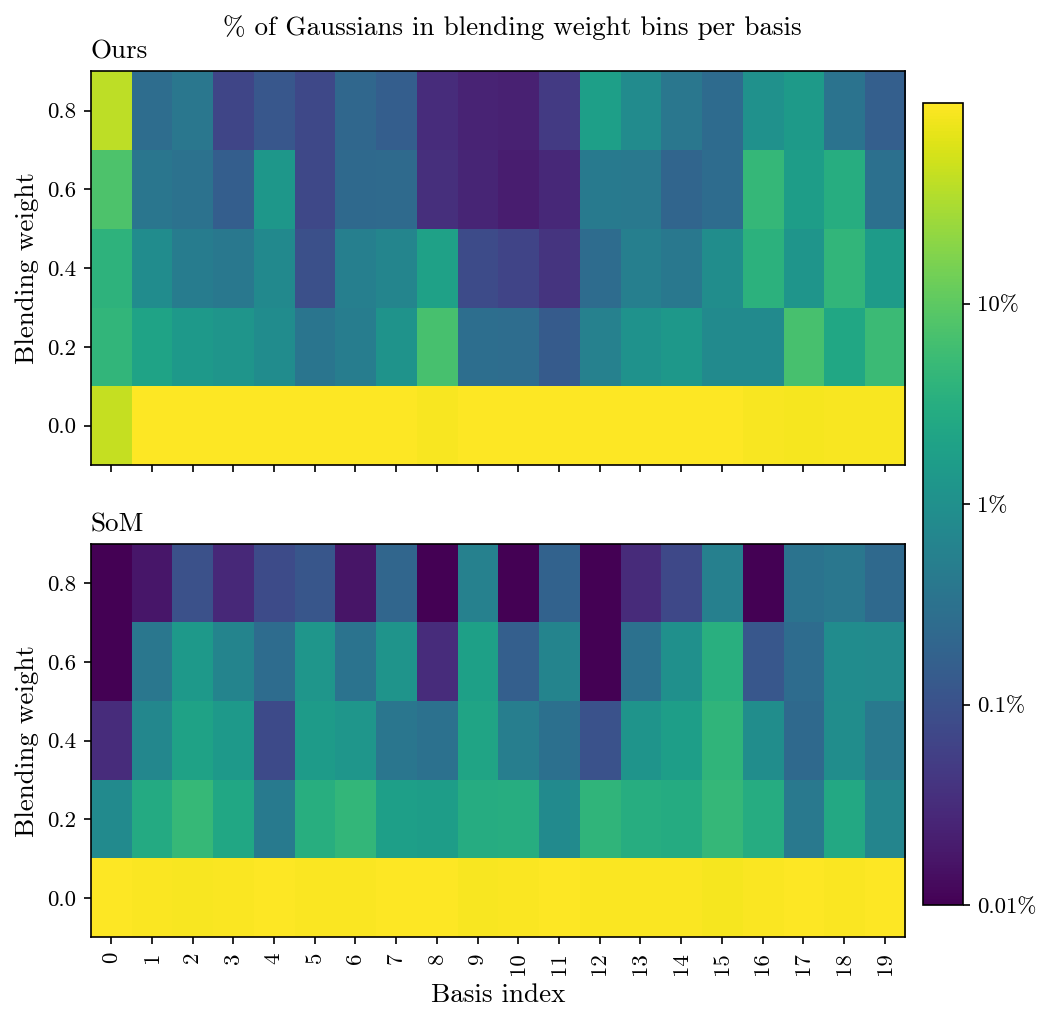
\includegraphics[width=\linewidth]{img/heatmap.png}
  \caption{Average Gaussian basis blending weights across bases.}
  \label{fig:basis-utilization-heatmap}
\end{figure}



%\subsection{Progressive Motion Addition}

%Motivated by this, we replace the fixed basis count $B$ with an adaptive scheme that grows bases where the motion model fails, using the photometric loss gradient as a densification signal, inspired by 3DGS densification~\cite{kerbl20233d}. We start by initializing only a single basis, following the initialization scheme in SoM~\cite{wang2025shape} using precomputed TAPIR~\cite{doersch2023tapir} tracks. Then optimize one basis at a time, freezing previously added bases so each new basis refines local motion without disturbing motion already captured.

%For each Gaussian $g$ with blending weight $w_g^{(b)}$ for basis $b$ and center $\mu_g$, we define its \textit{error contribution} to that basis as $e_g^{(b)} = w_g^{(b)} \lVert \partial \mathcal{L}_{\mathrm{RGB}} / \partial \mu_g \rVert_2^2$. Every few iterations, we compute the basis-level error $e^{(b)} = \sum_g e_g^{(b)} / \sum_g w_g^{(b)}$, the normalized sum of error contributions over all Gaussians, and flag $b$ for densification if $e^{(b)} > \tau$ ($\tau=10^{-5}$). Within a flagged basis, we take the top $15\%$ of Gaussians by error contribution and match each to its nearest TAPIR track in the canonical frame. A new basis is pre-trained on these tracks alone, with all other parameters frozen, using a per-track L2 loss weighted by TAPIR's confidence and visibility scores. We then unfreeze all motion and appearance parameters and jointly optimize against the photometric loss for 1500 steps until the next basis densification.

% ------ original version -------
% Rather than setting the number of motion bases B as a predetermined hyperparameter, our method instead grows the bases adaptively using the photometric loss gradient as a densification signal, inspired by the control steps in 3DGS~\cite{kerbl20233d}.
% We segment the moving part of the input video using SAM2~\cite{ravi2024sam2} and initialize with one cluster using KMeans clustering on track velocity and initialize the motion basis with Procrustes.
% This first transform represents the average motion of all tracks in the scene.

% After the initialization, We optimize one new basis at a time and freeze all previously added bases, so that each new basis refines local motion without disrupting the global rigid motion captured by earlier bases.
% This setup allows more transforms to be fitted to regions of complex motions dynamically and for the number of bases required to be tailored for each scene.

% \textbf{Notation.}
% Let $N$ be the number of foreground moving Gaussians, with optimizable parameters $(\mu_0, R_0, s, o, c)$.
% For the current set of $B$ active bases, let $w_g^{(b)}\!\in\![0,1]$ be the post-softmax coefficient of Gaussian $g$ on basis $b$.
% We write $t_0$ for the canonical frame, initialized as the frame with the highest number of visible tracks.

% \textbf{Adaptive Basis Densification} Every fixed number of iterations, we run adaptive densification on the bases.
% We evaluate the gradient of the basis cluster by taking every Gaussian's RGB loss against its mean weighted by the coefficient against the basis.
% \begin{equation}
%   e^{(b)} =
%   \frac{\displaystyle\sum_{g=1}^{N} w_g^{(b)}
%         \left\lVert \frac{\partial \mathcal{L}_{\mathrm{RGB}}}{\partial \boldsymbol{\mu}_g} \right\rVert_2^2}
%        {\displaystyle\sum_{g=1}^{N} w_g^{(b)}}\,.
%   \label{eq:basis-error}
% \end{equation}

% This per-cluster gradient is normalized by the total sum of coefficients belonging to the cluster such that the gradient magnitude is not affected by cluster size.
% A basis is flagged for densification when $e^{(b)} > \tau$, set to $1\times 10^{-5}$ empirically.

% For all bases to be densified, we localize the high-residual region by finding the per Gaussian gradient weighted by its coefficient to the cluster
% \begin{equation}
%   e_g^{(b)} = w_g^{(b)}
%   \left\lVert \frac{\partial \mathcal{L}_{\mathrm{RGB}}}{\partial \boldsymbol{\mu}_g} \right\rVert_2^2,
%   \label{eq:gaussian-error}
% \end{equation}
% to identity the top $15\%$ of high-gradient Gaussians for that cluster.
% As the Gaussians no longer have a 1-to-1 match to the TAPIR tracks after densification and culling, we associate them to the spatially nearest TAPIR tracks via k-nearest-neighbour query on the Gaussian means at the canonical frame compared to the pixel tracks.

% A new basis is fitted from the these tracks.
% This basis is pre-trained in a separate optimization loop from the main optimization, with all Gaussian parameters and all other bases frozen.
% The basis is optimized using a mean squared-error loss, weighted by the confidence and visibility scores on the tracks, between the predicted tracks $\hat{\mathbf{p}}_k$ and the TAPIR pseudo-GT tracks $\mathbf{p}_k$:
% \begin{equation}
%   \mathcal{L}_{\mathrm{track}} =
%   \sum_{k=1}^{K} \sum_{t} c_k^{(t)}\, v_k^{(t)}
%   \left\lVert \hat{\mathbf{p}}_k^{(t)} - \mathbf{p}_k^{(t)} \right\rVert_2^2\,,
%   \label{eq:track-loss}
% \end{equation}
% where $c_k^{(t)}\!\in\![0,1]$ and $v_k^{(t)}\!\in\!\{0,1\}$ are the TAPIR confidence and visibility scores of track $k$ at frame $t$.

% The pre-trained transform is added as the new basis, $\mathbf{T}^{(B+1)}_{0\to t}$, and its per-Gaussian coefficients are initialized by assigning each Gaussian to its nearest pseudo-GT track in the canonical frame.
% Then, the other parameters are unfrozen and the full scene reconstruction is optimized against the photometric loss.

% ------ Claude draft (2026-10-21; updated 2026-11-03, momo-modes study): the current default method (residual-driven basis
% splitting at initialisation with residual-pattern clustering and the squared residual, no child Gaussians; arm split_init).
% Until 2026-11-03 the default had no clustering and an L1 residual ("candidate default" in the experiment reports). It runs on
% the 3D tracks only and replaces SoM's initialisation; the subsection "Progressive Motion Addition" above
% describes the earlier photometric-gradient variant. -------
\subsection{Progressive Motion Addition}
\label{sec:split-init}

SoM initializes all $B$ bases at once: it clusters the 3D track velocities with $k$-means, fits one SE(3) trajectory per
cluster by Procrustes alignment and refines bases and blending weights jointly~\cite{wang2025shape}. We instead grow the
bases one at a time on the 3D tracks as a pretraining step before any photometric optimization. The first basis captures the average motion of
the scene. Each additional basis is split off the current worst basis, and is placed where it removes the most residual track error. 
The basis growth stops once an added basis lowers the total track error by less than a $\tau$ percentage cutoff.
After all bases are added, a final polishing step performs a joint optimization.
\paragraph{Motion model and tracks.}

A foreground Gaussian $g$ is defined to have a canonical center $\boldsymbol{\mu}_g$ at frame $t_0$ and blending weights
$\mathbf{w}_g = \operatorname{softmax}(\mathbf{l}_g)$ over the current $K$ bases. Its center at time $t$ is
\begin{equation}
  \boldsymbol{\mu}_g(t) = \Big(\sum_{b=1}^{K} w^{(b)}_g\, \mathbf{T}^{(b)}_{0\to t}\Big)\, \boldsymbol{\mu}_g ,
  \label{eq:blend}
\end{equation}
where the rotations are blended in the continuous 6D parameterization~\cite{zhou2019continuity} and mapped back to
SO(3). We follow \citep{wang2025shape} and initialize the Gaussian mean at a canonical time frame $t_0$ which has the highest number of visible tracks. Each Gaussian is initialized from a pseudo-ground truth 2D track lifted to 3D with depth and camera poses, giving a target
trajectory $\mathbf{p}_g(t)$ and a per-frame weight $\omega_g(t) = v_g(t)\, c_g(t)$ from the track's visibility $v_g(t)$
and confidence $c_g(t)$. We initialize with only one motion basis, fit over all the tracks using over a confidence- and visibility-weighted L1 loss. 

\paragraph{Residual and per-track error.}
After the fitting stage, the residual of track $g$ is $\mathbf{r}_g(t) = \boldsymbol{\mu}_g(t) - \mathbf{p}_g(t)$. We remove its
weighted temporal mean, since a Gaussian that follows its track at a constant offset has no motion error:
\begin{equation}
  \bar{\mathbf{r}}_g(t) = \mathbf{r}_g(t) - \frac{\sum_s \omega_g(s)\, \mathbf{r}_g(s)}{\sum_s \omega_g(s)} .
  \label{eq:residual}
\end{equation}
The error of track $g$ sums the residual distance over time,
\begin{equation}
  \varepsilon_g = \sum_t \omega_g(t)\, \big\lVert \bar{\mathbf{r}}_g(t) \big\rVert_2\claudeadd{^2} , \qquad
  \bar\varepsilon_g = \varepsilon_g \Big/ \sum_t \omega_g(t) ,
  \label{eq:track-error}
\end{equation}
the residual energy of the track.

\paragraph{Basis splitting decision.}
Basis $b$ is responsible for the error of the Gaussians that use it,
$S^{(b)} = \sum_g w^{(b)}_g\, \varepsilon_g$.
So that a handful of outlier tracks cannot attract a basis, the errors of the 10\,\% worst-fitted tracks are first capped at the 90th-percentile error.
We plan a split for each of the three bases
with the largest $S^{(b)}$.
The members $\mathcal{M}_b$ of basis $b$ are the Gaussians whose largest blending weight is on $b$. The \emph{candidates} are their poorly fitted half: the members whose mean error $\bar\varepsilon_g$ is at least the members' median. They may follow
several distinct motions, and a clone fitted to all of them would follow their average and blend the parts. We therefore
split the candidates by the \emph{pattern} of the residual: each residual trajectory $(\omega_g(t)\,\bar{\mathbf{r}}_g(t))_t$ is
normalized to unit length, reduced to 8 dimensions by PCA, and clustered by 2-means seeded by the sign of the first
principal component. The \emph{movers} $\mathcal{G}_b$ are the cluster with the larger mean error $\bar\varepsilon_g$, so each new basis
is fitted to one coherent motion (\eg a limb or one person) that the coefficients can then separate.
For each planned split, a new basis is fitted to the movers as described next, and its \emph{gain} is the resulting drop of the movers' error,
$\Delta_b = \sum_{g \in \mathcal{G}_b} (\varepsilon_g - \varepsilon'_g)$, where $\varepsilon'_g$ is the error of $g$ (\cref{eq:track-error}) once its trajectory is corrected by the new basis.
We keep the split with the largest gain.



% [Claude] 2026-11-05: "Procrustes-informed clone" and "Soft hand-off of coefficients" merged into "Initialize new basis" (user request).
% The detailed version with the two equations moved to sec/X_suppl.tex. Below, the old headings are commented out and the old text is
% struck; the two equations are left for you to delete, and their labels moved with the supplementary copy.
\paragraph{Initialize new basis.}
The new basis starts as a copy of basis $b$, composed with a per-frame rigid correction that best explains the movers' residual.
For every frame, the correction aligns the movers' current positions with their tracks, each shifted by its constant offset, by weighted Procrustes~\cite{umeyama1991least}; it is interpolated over frames where the movers are barely visible.
The members of $b$ then share their blending weights between $b$ and the new basis according to how well each basis explains them: the new basis receives a share given by a logistic function of the difference between the member's errors under the parent and under the clone.
The pair thus keeps the parent's total weight, and a Gaussian that both explain equally well is shared evenly instead of being assigned to one.
All other Gaussians receive a near-zero weight on the new basis.
\Cref{sec:suppl-init} gives the equations.




% [Claude] 2026-11-05: placeholder heading "Fitting Stage / Loss" replaced by the two paragraphs below (user request).
% \paragraph{Fitting Stage / Loss}
\paragraph{Fitting loss.}
Every fit, of the first basis and after each split, minimizes the initialization objective of SoM~\cite{wang2025shape} on the tracks.
Its main term is the confidence- and visibility-weighted $\ell_1$ distance between the predicted positions $\boldsymbol{\mu}_g(t)$ and the lifted tracks $\mathbf{p}_g(t)$.
It is complemented by an $\ell_1$ reprojection loss on the 2D tracks, a sparsity term that pushes each Gaussian's blending weights toward a single basis, and smoothness penalties on the accelerations of the bases and of the trajectories, including along the camera's depth axis.
Each fit updates the bases, the blending weights and the canonical centers with 200 iterations of Adam~\cite{kingma2014adam} at an exponentially decaying learning rate; the final polishing step runs 1000 iterations at a tenth of that learning rate.

\paragraph{Stopping criterion.}
\label{sec:tau}
After each fit we measure the scene's track error, the weighted mean distance between the predicted and the observed track positions,
\begin{equation}
  E_K = \frac{\sum_g \sum_t \omega_g(t)\, \lVert \mathbf{r}_g(t) \rVert_2}{\sum_g \sum_t \omega_g(t)} ,
  \label{eq:scene-error}
\end{equation}
where $K$ is the current number of bases.
The growth stops at the first split that lowers this error by less than a fraction $\tau$ of its previous value, $1 - E_K / E_{K-1} < \tau$.
We use $\tau = 0.05$ in all experiments. 





\lulu{Adam vs Gauss Newton ablation, first direct Pytorch solver then look into conjugate gradients}



